\paragraph{Main comparison.}
\Cref{tab:main} compares the memory with the baselines on all \nTestScenes{} test scenes. The definition alone (\emph{never split}) is right exactly on the \nWholeFam{} families that never come apart (\accNever\% of scenes). The memory reproduces the exact ground-truth partition of \accAll\% of scenes (95\% interval \accLo--\accHi\%), with PQ \pqAll\%: \accSingle\% of single objects, \accArranged\% of arrangements and \accWhole\% of things that never come apart. Logistic regression on the same traits and entries ranks true units about as well (its AUROC is higher) but its decision at $0.5$ splits almost everything: it finds more units and produces \fpLogistic{} false segments per scene against \fpLatent{} for the memory, and splits \splitWholeLogistic\% of things that never come apart against \splitWholeLatent\%. The boundary-contrast rule fares worse still (\accEdge\%): a strong edge is everywhere in these scenes---around a cap, but also around the painted band on a vase, a label on a book, the head of a hammer---and edges alone cannot tell which of them come apart. What separates the memory from both is not a better ranking but its abstention: a part is called separable only where enough stored parts that \emph{came away} sit nearby (\cref{prop:evidence}), and otherwise the definition's answer---one object---stands. Without the credible bound and support condition (\emph{no abstention}) accuracy falls to \accNoAbst\%.

\begin{table}[t]
\centering\small
\caption{Test scenes (\nTestPerFamily{} per family). Exact: share of scenes whose partition is reproduced exactly (95\% bootstrap interval); PQ: panoptic quality; unit recall: share of ground-truth units recovered; FP: false segments per scene; AUROC: ranking of true units among all candidates. All rows use the same candidates, selection and partition step.}
\label{tab:main}
\setlength{\tabcolsep}{4pt}
\begin{tabular}{@{}lrrrrrrrr@{}}
\toprule
 & \multicolumn{1}{c}{Exact (\%)} & PQ & single & arranged & whole & unit rec. & FP & AUROC \\
\midrule
\tabinput{tables/main.tex}
\bottomrule
\end{tabular}
\end{table}

\paragraph{Validated choices.} With the interactive application's original settings (relevance-weighted distance, $k=24$, $\theta_+=0.65$, $w_0=0.7$) the memory reaches \accDefault\%; the validated settings bring it to \accAll\%. Two of the changes are findings rather than tuning. First, weighting traits by their Fisher separation lowers accuracy (\accRelOn\% with the validated $k,\theta_+,w_0$). The weights it learns concentrate on the signal-edge traits (the largest: \relTop{}): parts that came away do have strong edges on average, so the criterion turns the distance into something close to an edge detector---and edges, as the boundary-contrast rule shows, are everywhere, including around parts that never come away. Equal weights keep the shape and contact traits in play, and those are what tell a cap from a painted band. Second, carried-whole entries are nearly worthless as evidence against separation (\cref{tab:ablation}): at their original weight $0.7$ accuracy on arrangements collapses to \arrCarriedSeven\%, because every carry of a bookshelf records book-shaped parts that stayed with it.

\paragraph{Candidate generators.} Straight cuts alone describe single objects well (\accCutsOnlySingle\% exact) but few of the arrangements (\arrCutsOnly\%); regions alone fail on single objects (\accRegionsOnlySingle\%, e.g.\ caps the colour of their body) and do better on arrangements (\arrRegionsOnly\%). Only their union does well on both.

\paragraph{Where it fails.} \Cref{fig:qualitative} shows predictions on test scenes. Over all separable families the memory recovers \unitsFound\% of the units. Arrangements are hard mostly because an exact partition needs \emph{every} unit: a test bookshelf holds up to \maxBooks{} books. Of the \arrMissed{} units missed in arrangements (out of \arrUnits), \missNotCalled\% had a candidate overlapping them well (IoU $\ge0.5$) that the memory did not call---it abstained for want of nearby parts that came away---\missNoCand\% had no such candidate at all (the generators did not propose the unit; \missNoCandShelf{} of these are books and \missNoCandCabinet{} drawers), and \missBadly\% were called but lost to an overlapping, worse-fitting candidate.

\begin{figure}[t]
\centering
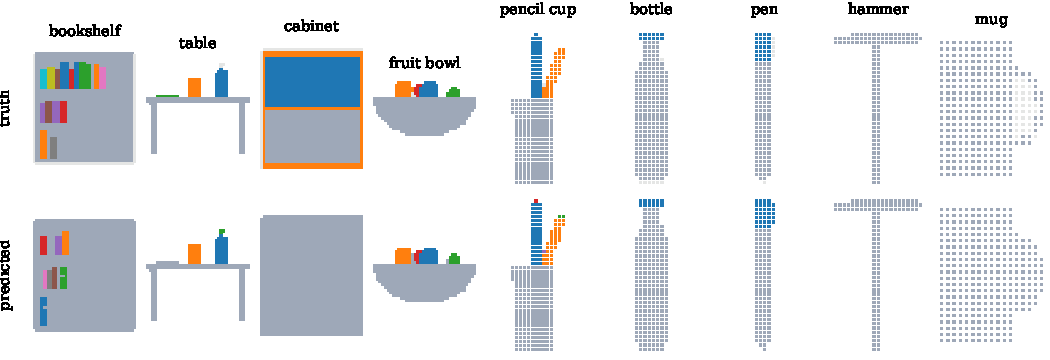
\includegraphics[width=\linewidth]{figures/qualitative.pdf}
\caption{Test scenes, nothing moved. Top: ground-truth partition (grey: void). Bottom: the memory's prediction (patches coloured by predicted object).}
\label{fig:qualitative}
\end{figure}

\paragraph{How much teaching.} \Cref{fig:curve} varies the number of handled scenes per family. Accuracy rises from \curveOne\% with one scene per family to \curveForty\% with \nTrainPerFamily{}, and has not levelled off. The gain is largest for single objects (\curveOneSingle\%$\to$\curveFortySingle\%), then arrangements (\curveOneArranged\%$\to$\curveFortyArranged\%). Things that never come apart start high (\curveOneWhole\%$\to$\curveFortyWhole\%): with nothing stored nearby that came away, the memory does not speak and the definition's answer stands; more teaching mainly removes the few false calls.

\begin{figure}[t]
\centering
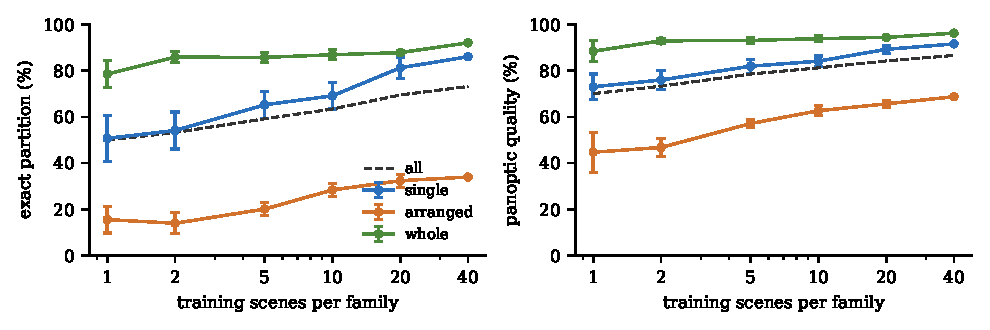
\includegraphics[width=\linewidth]{figures/curve.pdf}
\caption{Learning curves: exact-partition accuracy and PQ against the number of handled training scenes per family (mean $\pm$ s.d. over 5 random subsets).}
\label{fig:curve}
\end{figure}

\paragraph{New kinds of things.} \Cref{fig:lofo} removes each family from memory in turn and tests on it. Averaged over families, the memory reproduces \lofoMean\% of scenes of a family it has never seen (\lofoSingle\% for single objects, \lofoArranged\% for arrangements, \lofoWhole\% for things that never come apart), against \lofoMeanLogistic\% for logistic regression. Transfer between groups is weak: taught only single objects (and things that never come apart), it reproduces \trSA\% of arrangements; taught only arrangements, \trAS\% of single objects. Knowledge of what comes apart carries over between caps and lids of different single objects (a held-out single family is reproduced \lofoSingle\% of the time), but hardly between arrangements (\lofoArranged\%), and a book among books and a cap on a bottle are different enough in these traits that one does not teach the other. When a family is held out, the distance from its candidates to the nearest stored entry grows by a factor of \oodRatio{} (median), and the memory falls back on the definition.

\begin{figure}[t]
\centering
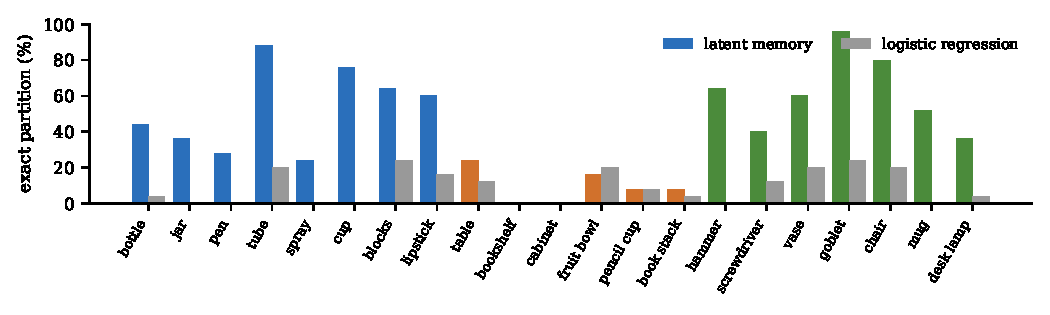
\includegraphics[width=\linewidth]{figures/lofo.pdf}
\caption{Leave-one-family-out: exact-partition accuracy on a family that is absent from memory (memory: all other families).}
\label{fig:lofo}
\end{figure}

\paragraph{Teaching a new kind.} \Cref{fig:fewshot} adds $k$ handled scenes of the held-out family to the memory of all others. Averaged over separable families, accuracy goes from \fsZero\% at $k=0$ to \fsTen\% at $k=10$ (single objects \fsZeroSingle\%$\to$\fsTenSingle\%, arrangements \fsZeroArranged\%$\to$\fsTenArranged\%). Consistent with \cref{prop:evidence}, one or two scenes change nothing on average (\fsOne\% and \fsTwo\%); five do (\fsFive\%). The memory states \emph{separates} only with three entries' worth of evidence nearby, and one handled scene contributes one to three. Families that never come apart gain too (right panel), although their carried-whole entries count almost nothing as evidence: what they change is \emph{who the neighbours are}. Once a few hammers are stored, a hammer's candidates find hammers among their $k=\chosenK$ nearest entries instead of distant parts that came away, and the memory stops calling separations it has no support for.

\begin{figure}[t]
\centering
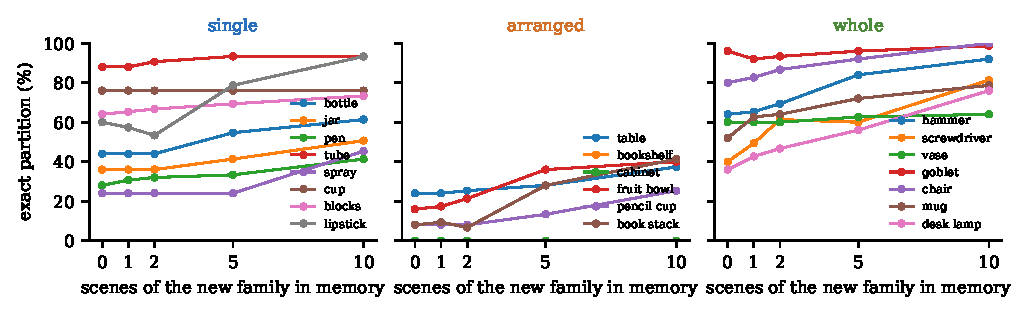
\includegraphics[width=\linewidth]{figures/few_shot.pdf}
\caption{Few-shot teaching of a family that was absent from memory: accuracy after adding $k$ handled scenes of it (mean over 3 random draws).}
\label{fig:fewshot}
\end{figure}

\paragraph{Ablations.} \Cref{tab:ablation} removes or isolates trait groups and varies the validated settings. \ablationText

\begin{table}[t]
\centering\small
\caption{Ablations on the test scenes (exact-partition accuracy and PQ, \%). Trait groups as in \cref{tab:traits}.}
\label{tab:ablation}
\begin{tabular}{@{}lrrrrr@{}}
\toprule
 & Exact & PQ & single & arranged & whole \\
\midrule
\tabinput{tables/ablation.tex}
\bottomrule
\end{tabular}
\end{table}

\paragraph{Robustness.} \Cref{tab:robust} applies changes never seen in training. A hue shift and dimmer light leave accuracy unchanged (\robRecolour\% and \robDark\%), as \cref{prop:invariance} predicts: only signal changes, normalised by the object's own, enter the traits. Turning pictures by $90^\circ$ costs some accuracy (\robRotNinety\%) and by $180^\circ$ much more (\robRotOneEighty\%): every trait but \emph{above} is invariant, and the drop shows how much the memory relies on parts resting on top of what they come away from. Shrinking to $0.7\times$ (\robScale\%) leaves fewer patches per part, near the resolution of the sensing. Sensor noise hurts most (\robNoise\%). Noise raises every neighbour difference, and with it the object's own typical difference that normalises the signal traits, so edges stand out less; it also fragments regions of similar signal. We have not separated these two effects. Under noise, logistic regression is as good as the memory (\robNoiseLogistic\%): a plausible reason, which we have not tested, is that noise makes candidates look unlike anything stored, so the memory abstains where a linear rule still extrapolates.

\begin{table}[t]
\centering\small
\caption{Robustness: test scenes changed in ways never seen in training (\nRobustPerFamily{} scenes per family).}
\label{tab:robust}
\begin{tabular}{@{}lrrrrrr@{}}
\toprule
 & \multicolumn{4}{c}{latent memory} & \multicolumn{2}{c}{logistic} \\
\cmidrule(lr){2-5}\cmidrule(lr){6-7}
change & Exact & PQ & arranged & whole & Exact & PQ \\
\midrule
\tabinput{tables/robust.tex}
\bottomrule
\end{tabular}
\end{table}

\paragraph{Calibration.} With the original settings, $\hat p$ is well calibrated as the probability that a candidate is a true unit (ECE \eceOriginal{}, \cref{fig:calibration}); with the validated settings it is not (ECE \eceChosen{}). The base rate is low---\baseRate\% of candidates are true units---and with carried-whole entries counting almost nothing, $\hat p$ in a neighbourhood without positives stays near the prior's $0.5$. Accuracy and calibration pull in different directions here: the validated memory decides well because it decides only with support, but its $\hat p$ should be read as the share of nearby \emph{weighted} evidence, not as a calibrated probability.

\begin{figure}[t]
\centering
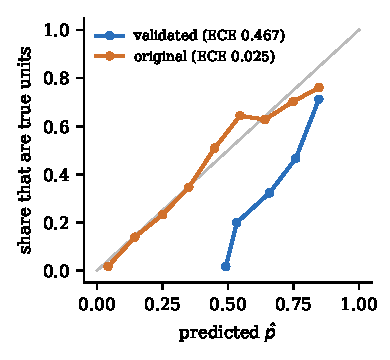
\includegraphics[width=0.45\linewidth]{figures/calibration.pdf}\hfill
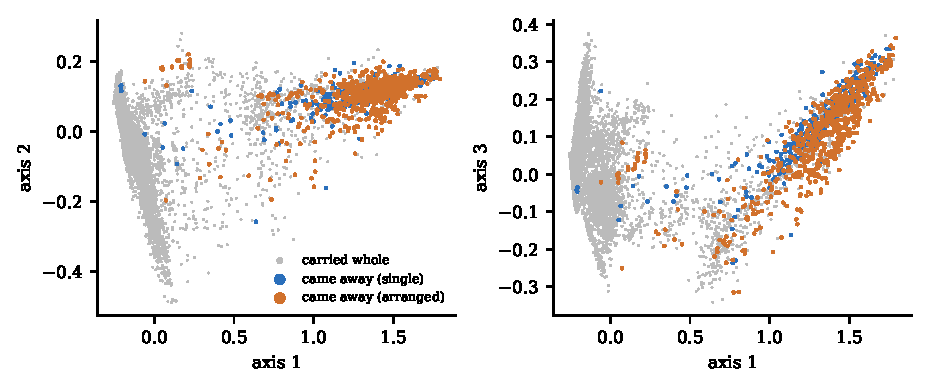
\includegraphics[width=0.53\linewidth]{figures/latent.pdf}
\caption{Left: reliability of $\hat p$ over all candidates of all test scenes (label: the candidate is a true unit, IoU $\ge0.75$). Right: the stored entries in the three directions of greatest spread of the standardised trait space; parts that came away (colour) occupy their own region, separate from parts that were carried whole (grey), for single objects and arrangements alike.}
\label{fig:calibration}
\end{figure}

\paragraph{Faithfulness of the evaluation.} The live session (the same code as the interactive application) with the full memory predicted exactly the partition the offline scoring computes on all \nEquivTotal{} test scenes we checked (\nEquivAgree{}/\nEquivTotal{}).
